\chapter{Introduction}
\vspace*{0.5cm}
\setcounter{page}{1}
\pagenumbering{arabic}

%Since the start of 2020 \textit{Sars-COVID19} has initiated a world-wide pandemic. In an attempt to slow down the fast and uncontrollable spread of this disease various prevention and diagnosis methods have been developed. In this work, out of all these various methods, the attention is going to be put on the possible developement diagnostic methods related to medical images, be they automatic or semi-automatic, to be intended either as Clinical Decision Support Systems (CDSS) or as a quick evaluation to completely avoid human analysis.
%In this light this first introductory chapter is going to start from a basic theoretical overview of the necessary core concepts that will be needed throughout this whole work such as definition of an image and imaging methods, with particular attention to those used in the medical field. This will be followed by an introduction to Artificial Intelligence (AI) and some Machine Learning techniques. Finally some of the concepts from the two previous topics will be treated jointly under the discipline of radiomics, which will be defined and explored as necessary.

Nowadays everybody knows of  \textit{Sars-COVID19} which, since the start of 2020, has made necessary a few world-wide quarantines forcing everybody in self-isolation. It is also well known that, among the main complications and features of this virus, symptoms gravity as well as the rate of deterioration of the conditions are some of the most relevant and problematic. In some cases asymptomatic or near to asymptomatic people may, in the span of a week, get to conditions that require hospital admission. This peculiarity is also what heavily complicates the triage process, since trying to predict with some degree of accuracy the prognosis of the patient at admission is a thoroughly complex task. In this thesis the aim will be to use data, specifically including data that cannot be easily interpreted by humans, to try various methods to predict a couple of clinical outcomes, namely the death of the patient or the admission in the Intensive Care Unit (ICU), while assessing their performance. These analyses will be carried out on a dataset of 434 patients with different variables associated to every person. A part of the variables, which will be called clinical and radiological, are defined by humans and are generally discrete in nature but mostly boolean. The most part of the available variables, however, will be image-derived following the approaches used in the field of radiomics. While the utility of clinical variables, such as age, obesity and history of smoking, is very straightforward it's interesting and helpful to understand the basis behind the utility of radiomic and radiological features.
Generally speaking it's clear that images have the ability to convey a slew of useful images, this is expecially true in the medical field where digital images are used to inspect also the internal state of the patient giving far more detailed information than that obtainable by visual inspection at the hand of medical professionals. Among the ways in which \textit{Sars-COVID19} can manifest himself the one that is most relevant to the scopes of this thesis pneumonia and the complications that stem from it. Some of these complications, which are not specific of \textit{Sars-COVID19} but can happen in any pneumonia case, display very peculiar patterns when visualizing the lungs through CT exams.
These patterns are due to the pulmonary response to inflammation which may lead to thickening of the bronchial and alveolar structures up to pleural effusions and collapsed lungs. Without going too much in clinical detail what is of interest is how these condition manifest themselves in the CT exams:

\begin{enumerate}
        \item \textbf{Ground Glass Opacity(GGO)}:\newline Small diffused changes in density of the lung structure cause a hazy look in the affected region. This complicates the individuation of pulmonary vessels.
			\begin{figure}[htbp]
				\centering
				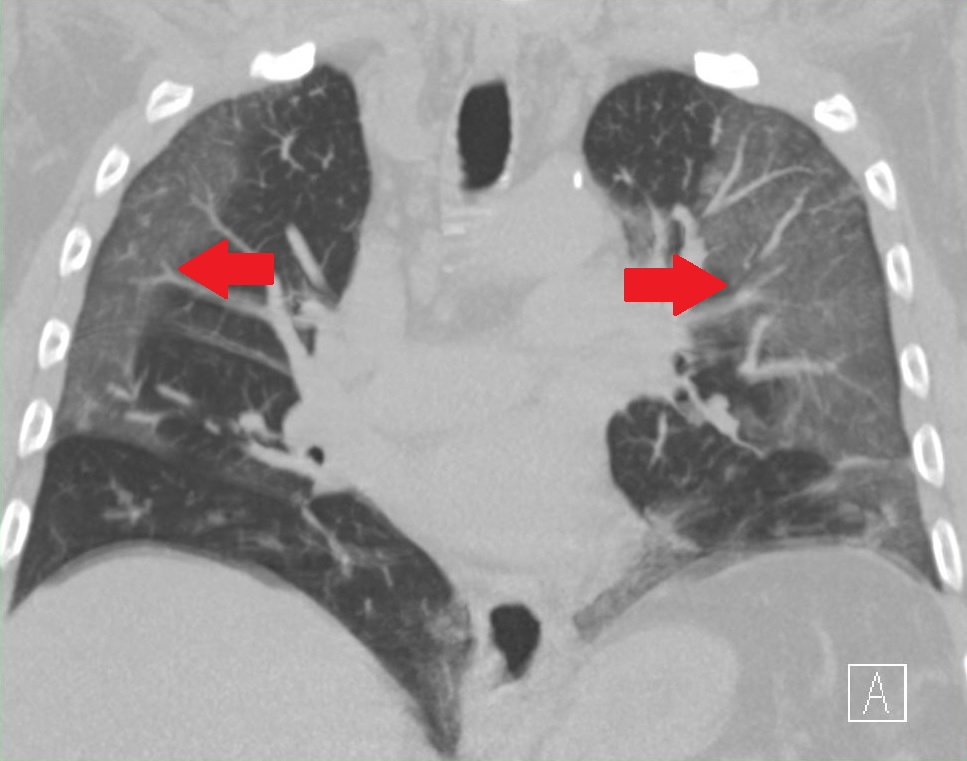
\includegraphics[width=0.66\linewidth]{GGO.jpg}
				\caption{Example of GGO\label{GGOImage}}
			\end{figure}
        \item \textbf{Lung Consolidations}:\newline Heavier damage reflects in whiter spots in the lung as the surface more closely resembles outside tissue instead of normal air. The consolidation refer to presence of fluid, cells or tissue in the alveolar spaces	
        \item \textbf{Crazy paving}:\newline When GGOs are superimposed with inter-lobular and intra-lobular septal thickening.
			\begin{figure}[htbp]
				\centering
				\subfloat[][a]{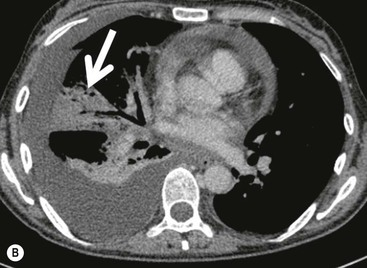
\includegraphics[width=0.35\linewidth]{CollapsedLung.jpg}}
				\subfloat[][a]{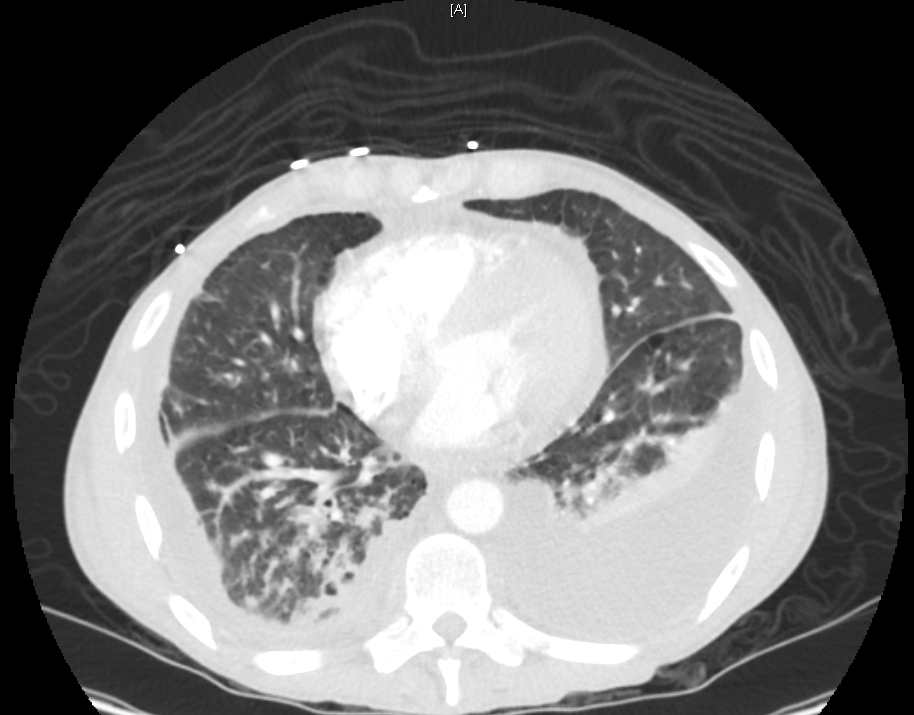
\includegraphics[width=0.33\linewidth]{PleuralEffusion.png}}
				\caption{Differences between a collapsed lung (a) and pleural effusion(b)}
			\end{figure}
	\item \textbf{Collapsed Lungs and Pleural Effusion}:\newline Both of these manifest themself as regions of the lungs that take the same coloring as that of tissue outside the lung. The main difference between the two is that collapsed lungs are somewhat rigid structures, they can occur in singular lobes of the lung and stay where they occur. Pleural effusions, however, are actually fluid being located in the lung instead of air. As such these lesions usually are located 'at the bottom' of the lung in which they happen and migrate to the lowest part of the lung according to the position of the patient.
\end{enumerate}

Having these manifestation it's clear that they are mainly textural and intensity-like changes in the normal appearance of the lungs. However, whereas these properties can be easily described in a qualitative and subjective way, it's rather complex to describe them in a quantitative and objective way. The field of radiomics, when coupled with digital images and preprocessing steps which must include image segmentation, is exactly what undertakes this daunting task. Radiomics comes from the the combination of radiology and the suffix \textit{-omics}, which is characteristic of high-throughput methods that aim to generate a large number of numbers, called biomarkers or features, as such it uses very precise and strict mathematical definitons to quantify in various ways either shape, textural or intensity based properties of the radiological image under analysis.
Given the large numerosity of the features produced by radiomics it's necessary to analyze these kinds of data with methods that rely on Machine Learning and their ability to address high-dimensional problems, be it in a supervised or unsupervised way, in a rather fast and accurate way.
Starting from these premises this thesis will be divided in a few chapters and sections. The first step will be taken by providing the general theoretical background regarding the aforementioned topics and techniques, this will be followed by a desscription of the data in use as well as a presentation of the analysis methods and resources used. Finally the results of the methods described will be presented and from them a set of concluding remarks will be set forth.
